\documentclass[12pt]{article}
\usepackage[top=1in, bottom=1in, left=1in, right=1in]{geometry}

\usepackage{setspace}
\onehalfspacing

\usepackage{amssymb}
%% The amsthm package provides extended theorem environments
\usepackage{amsthm}
\usepackage{epsfig}
\usepackage{times}
\renewcommand{\ttdefault}{cmtt}
\usepackage{amsmath}
\usepackage{graphicx} % for graphics files
\usepackage{tabu}

% Draw figures yourself
\usepackage{tikz} 

% writing elements
\usepackage{mhchem}

\usepackage{paralist}

% The float package HAS to load before hyperref
\usepackage{float} % for psuedocode formatting
\usepackage{xspace}

% from Denovo Methods Manual
\usepackage{mathrsfs}
\usepackage[mathcal]{euscript}
\usepackage{color}
\usepackage{array}

\usepackage[pdftex]{hyperref}
\usepackage[parfill]{parskip}

% math syntax
\newcommand{\nth}{n\ensuremath{^{\text{th}}} }
\newcommand{\ve}[1]{\ensuremath{\mathbf{#1}}}
\newcommand{\Macro}{\ensuremath{\Sigma}}
\newcommand{\rvec}{\ensuremath{\vec{r}}}
\newcommand{\vecr}{\ensuremath{\vec{r}}}
\newcommand{\omvec}{\ensuremath{\hat{\Omega}}}
\newcommand{\vOmega}{\ensuremath{\hat{\Omega}}}
\newcommand{\even}{\ensuremath{\phi^g}}
\newcommand{\odd}{\ensuremath{\vartheta^g}}
\newcommand{\evenp}{\ensuremath{\phi^{g'}}}
\newcommand{\oddp}{\ensuremath{\vartheta^{g'}}}
\newcommand{\Sn}{\ensuremath{S_N} }
\newcommand{\Ye}[2]{\ensuremath{Y^e_{#1}(\vOmega_#2)}}
\newcommand{\sigg}[1]{\ensuremath{\Macro^{gg'}_{s\,#1}}}
\newcommand{\psig}{\ensuremath{\psi^g}}
%---------------------------------------------------------------------------
%---------------------------------------------------------------------------
\begin{document}
\begin{center}
{\bf NE 255, Fa16 \\
Simplified P$_N$ Equations\\
October 04, 2016}
\end{center}

\setlength{\unitlength}{1in}
\begin{picture}(6,.1) 
\put(0,0) {\line(1,0){6.25}}         
\end{picture}

In slab geometry the P$_N$ equations can be written as a system of 1-D diffusion equations; this is not true in general geometry.
This if the motivation behind the simplified P$_N$ equations: what would happen if the P$_N$ method in general geometry was as nice as it is in slab geometry?

Gelbard introduced the SP$_N$ equations in a series of papers in 1962; however, they were not widely accepted as an approximate transport method because of the lack of a true theoretical foundation.
For approximately 30 years, the SPN equations were occasionally mentioned
in American Nuclear Society conference talks and brief publications.
It was not until the early 1990’s that theoretical work was published demonstrating that the SP$_N$ approximations have a valid mathematical foundation, and can be derived from either an asymptotic or a variational analysis.

\subsection*{``Heuristic'' Derivation of the SP$_N$ Equations}

Consider the planar (slab) geometry P$_N$ equations as before: for $l' = 0, 1, \dots$, we have
\[
\left(\frac{l'+1}{2l'+1}\right)\frac{d}{d x}\phi_{l'+1}(x) + \left(\frac{l'}{2l'+1}\right)\frac{d}{d x}\phi_{l'-1}(x) + \Sigma_t(x) \phi_{l'} = \Sigma_{sl'}(x)\phi_{l'}(x) + s_{l'}(x)\:,
\]
with $\phi_{-1}=0$ and
\[\phi_{N+1} = 0 \quad\text{ or }\quad\frac{d}{dx}\phi_{N+1}=0\,.
\]

The second-order form of the planar geometry P$_1$ equations with Marshak boundary conditions is the diffusion equation
\begin{align*}
&-\frac{d }{dx}D\frac{d \phi_0}{dx} + \Sigma_a(x) \phi_0(x) = s_0(x)\:, 0<x<X\,,\\
&\frac{1}{2}\phi_0(0)-D\frac{d\phi_0}{dx}(0) = 2J^+(0),\\
&\frac{1}{2}\phi_0(X)+D\frac{d\phi_0}{dx}(X) = 2J^-(X),
\end{align*}
where
\[
D = \frac{1}{3\left[\Sigma_t(x) - \Sigma_{s1}(x)\right]}.
\]

This can be generalized to 3-D by making the two \textbf{formal} modifications: 
\begin{enumerate}
\item Replace the 1-D diffusion operator 
\[
\frac{d }{dx}D\frac{d }{dx}
\]
by the 3-D diffusion operator
\[
\nabla\cdot D\nabla \equiv \frac{\partial }{\partial x}D\frac{\partial }{\partial x}+\frac{\partial }{\partial y}D\frac{\partial }{\partial y}+\frac{\partial }{\partial z}D\frac{\partial }{\partial z}\,;
\]
\item In the boundary conditions, replace the derivative terms
\[
\pm\frac{d }{dx}
\]
by the outward normal derivative
\[
\vec{n} \cdot \nabla
\]
\end{enumerate}
Making these formal modifications, we obtain the standard 3-D diffusion (P$_1$) equations
\begin{align*}
&-\nabla\cdot D\nabla\phi_0(\vecr) + \Sigma_a(\vecr) \phi_0(\vecr) = s_0(\vecr)\:, \vecr \in V,\\
&\frac{1}{2}\phi_0(\vecr)+D\vec{n}\cdot\nabla\phi_0 = 2J^-(\vecr), \, \vecr\in \partial V\,.
\end{align*}
These equations obviously reduce to the standard 1-D diffusion equations in planar geometry.

We carry out the same procedure for the general SP$_N$ equations. First, for odd values of $l'$, $\phi_{l'}$ is replaced by a vector:
\[
\phi_{l'} \rightarrow \vec{\phi}_{l'} = (\phi_{l'}^x,\phi_{l'}^y,\phi_{l'}^z)^t\,.
\]
Then, in the even $l'$ equations the derivative in $x$ is replaced by a divergence: 
\[
\frac{d}{dx} \rightarrow \nabla \cdot\,;
\]
and in the odd $l'$ equations the x derivative is changed to a gradient: 
\[
\frac{d}{dx} \rightarrow \nabla
\]
This allows us to write the first-order form of the SP$_N$ equations as 
\begin{align*}
&\nabla \cdot \vec{\phi}_1 + \Sigma_a\phi_0 = s_0\,,&&\\
&\left(\frac{l'+1}{2l'+1}\right)\nabla\phi_{l'+1} + \left(\frac{l'}{2l'+1}\right)\nabla\phi_{l'-1} + \Sigma_t \vec{\phi}_{l'} = \Sigma_{sl'}\vec{\phi}_{l'} + s_{l'}\:, & \text{for odd $l'$,}&\\
&\left(\frac{l'+1}{2l'+1}\right)\nabla\cdot\vec{\phi}_{l'+1} + \left(\frac{l'}{2l'+1}\right)\nabla\cdot\vec{\phi}_{l'-1} + \Sigma_t \phi_{l'} = \Sigma_{sl'}\phi_{l'} + s_{l'}\:, &\text{for even $l'>0$.}&
\end{align*}
The boundary conditions for the SP$_N$ equations can be obtained from the P$_N$ Marshak boundary conditions by replacing $\phi_{l'}$ with the SP$_N$ unknowns and $\mu$ with $\vec{n}\cdot\omvec$, where $\vec{n}$ is the unit inward normal to the boundary.

\subsection*{The SP$_3$ Equations}

Assuming an isotropic source, the SP$_3$ equations in their first-order form are
\begin{align*}
\nabla\cdot\vec{\phi}_1 + \Sigma_a\phi_0 &= s_0\,,\\
\frac{1}{3}\nabla\phi_0 + \frac{2}{3}\nabla\phi_2 + [\Sigma_t-\Sigma_{s1}]\vec{\phi}_1 &= 0\,,\\
\frac{2}{5}\nabla\cdot\vec{\phi}_1 + \frac{3}{5}\nabla\cdot\vec{\phi}_3 + [\Sigma_t-\Sigma_{s2}]\phi_2 &= 0\,,\\
\frac{3}{7}\nabla\phi_2 + [\Sigma_t-\Sigma_{s3}]\vec{\phi}_3 &= 0\,.
\end{align*}
We can rewrite them in their second-order form by using the relation
\[
\vec{\phi}_{l'} = -\frac{1}{\Sigma_t-\Sigma_{sl'}}\left(\frac{l'}{2l'+1}\nabla\phi_{l'-1}+\frac{l'+1}{2l'+1}\nabla\phi_{l'+1}\right)\,,
\]
yielding
\begin{align*}
&-\nabla \cdot \frac{1}{3[\Sigma_t-\Sigma_{s1}]}\nabla\phi_0
-\nabla \cdot \frac{2}{3[\Sigma_t-\Sigma_{s1}]}\nabla\phi_2
+\Sigma_a\phi_0 = s_0\,,\\
&-\nabla \cdot \frac{2}{15[\Sigma_t-\Sigma_{s1}]}\nabla\phi_0
-\nabla \cdot \left(\frac{4}{15[\Sigma_t-\Sigma_{s1}]}+\frac{9}{35[\Sigma_t-\Sigma_{s3}]}\right)\nabla\phi_2
+[\Sigma_t-\Sigma_{s2}]\phi_2 = 0\,.
 \end{align*}
The second-order form is useful because it makes the SP$_N$ equations look like a set of coupled diffusion equations. 

The SP$_3$ equations can be manipulated into a form that resembles a two group diffusion equation by defining $\hat\phi_0 = \phi_0+2\phi_2$.
Using this new variable, we can write
\begin{align*}
&-\nabla \cdot \frac{1}{3[\Sigma_t-\Sigma_{s1}]}\nabla\hat\phi_0
+\Sigma_a\hat\phi_0 = 2\Sigma_a\phi_2 + s_0\,,\\
&-\nabla \cdot \frac{9}{35[\Sigma_t-\Sigma_{s3}]}\nabla\phi_2
+ \left([\Sigma_t-\Sigma_{s2}]+\frac{4}{5}\Sigma_a\right)\phi_2
+ = \frac{2}{5}\left[\Sigma_a\hat\phi_0-s_0\right]\,.
 \end{align*}
These equations can be solved with a two-group diffusion code by properly setting the diffusion coefficients and cross-sections or with a one-group diffusion code utilizing an iteration strategy for the coupling terms (FLIP).

\subsection*{General Properties of the SP$_N$ Equations}

The SP$_N$ equations can be understood as a ``super'' diffusion theory.
The structure of the SP$_N$ equations is that of a coupled system of diffusion equations, and the class of problems for which the SP$_N$ equations are accurate encompasses the class of problems for which diffusion theory is accurate.

\begin{enumerate}
\item In 1-D planar geometry, SP$_N$ and P$_N$ are identical
\item In multidimensional problems, SP$_N$ form a system of (N + 1) equations; P$_N$ form a much larger system of (N + 1)$^2$ equations
\item The SP$_N$ equations have the same ``diffusion'' (elliptic) structure as the P$_1$ equations; the P$_N$ equations have a more complicated (hyperbolic) mathematical structure.
\item The above derivation of the SP$_N$ equations assumes as its starting point a 1-group transport problem.
However, applying the same procedures to a multigroup transport problem is straightforward.
The only complication is that the diffusion coefficients can become non-diagonal matrices.
Thus, unlike standard multigroup diffusion theory (but like standard multigroup P$_1$ theory), the multigroup SP$_N$ equations generally have non-diagonal matrix diffusion coefficients.
\item In principle, the 2-D or 3-D SP$_N$ equations can be implemented in a 2-D or 3-D diffusion code without fundamentally rewriting the code.
This is not the case for the P$_N$ equations.
\item The SP$_N$ equations contain more ``transport physics'' than the diffusion equations.
For this reason, solutions of the SP$_N$ equations can contain boundary layers that are not present in P$_1$ solutions.
In order to properly resolve these boundary layers, it may be necessary to use a finer spatial grid for the SP$_N$ equations than for the diffusion equation.
Alternatively, the use of nodal methods with extra expansion terms capable of expressing the boundary layer effects may be required.
\item The multigroup SP$_3$ equations are about twice as costly to solve as the multigroup P$_1$ equations.
However, SP$_3$ solutions are usually much more accurate (transport-like) than P$_1$ solutions.
\item In the limit as $N\rightarrow\infty$, the P$_N$ solutions converge to the transport solution.
\item In the limit as $N\rightarrow\infty$, the SP$_N$ solutions do not generally converge to the transport solution--unless the underlying problem is 1-D.
Therefore, high-order SP$_N$ equations cannot be used to obtain arbitrarily accurate solutions of neutron transport problems in 2 or 3 dimensions.
\item For 3-D problems, the system of P$_N$ equations is much more complicated in structure and greater in number than the system of SP$_N$ equations.
Also, for problems having 1D symmetry, the P$_N$ and SP$_N$ equations become identical.
For these reasons, it is widely believed that the 3-D SP$_N$ equations can be derived by discarding the proper terms (and equations) from the 3D P$_N$ equations. However, this has never been shown.
In fact, the precise relationship between the 3D P$_N$ and the 3D SP$_N$ equations is not known.
\item For problems in which the P$_1$ solution is accurate, the SP$_3$ solution is generally much more accurate.
As problems become less ``diffusive'' (absorption, streaming, or leakage become increasingly important), the P$_1$ and SP$_3$ solutions both degrade in accuracy.
However, the P$_1$ solutions degrade more rapidly, and the SP$_3$ solutions can
remain accurate well into the range in which P$_1$ solutions are not accurate.
When the problem becomes sufficiently ``difficult'', the P$_1$ and SP$_N$ solutions both become inaccurate (see figure in the next page).
\end{enumerate}

\newpage

\begin{center}
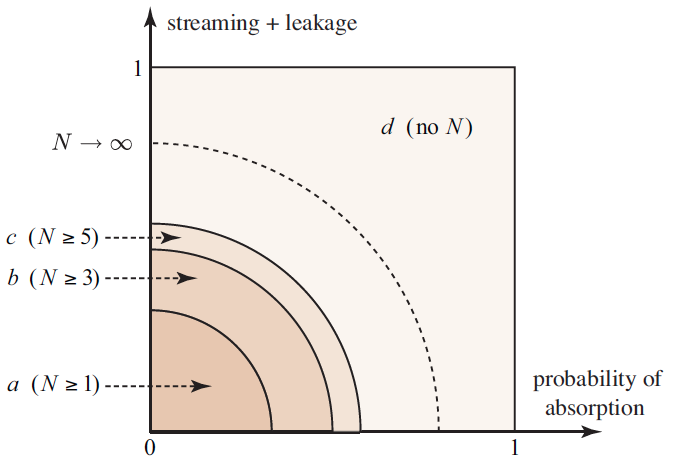
\includegraphics[scale=0.7]{fig_spn}
\end{center}

This figure shows the (qualitative) range of validity of the SP$_N$ equations.
The amounts of absorption and streaming/leakage are indicated on arbitrary scales ranging from 0 to 1.
In region $a$, where streaming, leakage, and absorption are weak, the P$_1$ and all SP$_N$ solutions are accurate.
As absorption or streaming increase (region $b$), P$_1$ becomes inaccurate but SP$_N$ with $N \geq 3$ is still accurate.
As absorption or streaming increase further (region $c$), P$_1$ and SP$_3$ are inaccurate but SP$_N$ with $N \geq 5$ is still accurate.
In region $d$, no SP$_N$ solution is accurate.

--------------------------

\vfill

These notes are derived from Edward Larsen's class notes for NE 644 at the University of Michigan, and from Ryan McClarren's review paper on the SP$_N$ equations: ``Theoretical Aspects of the Simplified P$_n$ Equations'', Transport Theory and Statistical Physics 39: 73--109, 2011.


\end{document}
Contact GitHub 